%%%%%%%%%%%%%%%%%%%%%%%%%%%%%%%
%%%%%%%%%%%%%%%%%%%%%%%%%%%%%%%
\chapter{Ship rigid body dynamics models}
\label{ch:models}
%%%%%%%%%%%%%%%%%%%%%%%%%%%%%%%

The ship's dynamics comprises the forces and motions in the six degrees of freedoms (6DOF): surge, sway, heave, roll, pitch and yaw. Heave and pitch motions are often neglected in calm water conditions, so that a four degrees of freedom (4DOF) model is sufficient to express the ship's dynamics. Models for roll and the manoeuvring model for the remaining DOFs are presented in section \ref{sec:roll} and section \ref{sec:manoeuvring model}. 

\section{Roll motion} \label{sec:roll}

The roll motion without manoeuvres in calm water with no external forces can be expressed with Eq.\ref{eq:roll_decay_equation_general_himeno} \cite{himeno_prediction_1981},
\begin{equation} \label{eq:roll_decay_equation_general_himeno}
A_{44} \ddot{\phi} + \operatorname{B_{44}}\left(\dot{\phi}\right) + \operatorname{C_{44}}\left(\phi\right) = 0
\end{equation}


\noindent where $B_{44}\left(\dot{\phi}\right)$ can be expressed as expansion series:  
$ B_{44}\left(\dot{\phi}\right) = B_1\cdot\dot{\phi} + B_2\cdot\dot{\phi}\left|\dot{\phi}\right| + B_3\cdot\dot{\phi}^3 + ... + B_n\cdot\dot{\phi}^n$. Most often, the so-called ``linear model'' (Eq.\ref{eq:roll_decay_equation_himeno_linear}), ``quadratic model'' (Eq.\ref{eq:roll_decay_equation_himeno_quadratic_b}) and ``cubic model'' (Eq.\ref{eq:roll_decay_equation_cubic}) are used to represent $B_{44}(\dot{\phi})$ by truncating the series to keep only linear, quadratic and cubic terms,

\begin{equation} \label{eq:roll_decay_equation_himeno_linear}
A_{44} \ddot{\phi} + B_{1} \dot{\phi} + C_{1} \phi = 0
\end{equation}

\begin{equation} \label{eq:roll_decay_equation_himeno_quadratic_b}
A_{44} \ddot{\phi} + C_{1} \phi + \left(B_{1} + B_{2} \left|{\dot{\phi}}\right|\right) \dot{\phi} = 0
\end{equation}

\begin{equation} \label{eq:roll_decay_equation_cubic}
A_{44} \ddot{\phi} + \left(B_{1} + B_{2} \left|{\dot{\phi}}\right| + B_{3} \dot{\phi}^{2}\right) \dot{\phi} + \left(C_{1} + C_{3} \phi^{2} + C_{5} \phi^{4}\right) \phi = 0
\end{equation}


\section{Vessel Manoeuvring Models} \label{sec:manoeuvring model}
\label{\detokenize{02.01_manoeuvring models:vessel-manoeuvring-models}}\label{\detokenize{02.01_manoeuvring models:vmm}}\label{\detokenize{02.01_manoeuvring models::doc}}
Ship manoeuvring is a simplified case of seakeeping. The encountering waves have been removed, assuming calm water conditions. The manoeuvring motions have low frequencies so that added masses and other hydrodynamic derivatives can be assumed as constants  \cite{fossen_handbook_2021}. Three manoeuvring models are used in this thesis: 
\begin{itemize}
    \item Linear (LVMM) \cite{matusiak_dynamics_2017}
    \item Abkowitz (AVMM), \cite{abkowitz_ship_1964}
    \item Modified Abkowitz (MAVMM), which is proposed in Paper \ref{pap:pit}
\end{itemize}

\noindent\autoref{\detokenize{02.01_manoeuvring models:coordinate-system}} shows the reference frames used in the manoeuvring models where \(x_0\) and \(y_0\) and heading \(\Psi\) are the global position and orientation of a ship fix reference frame \(O(x,y,z)\) (or rather \(O(x,y)\) when heave is excluded) with origin at midship. \(u\), \(v\), \(r\), \(X\), \(Y\) and \(N\) are velocities and forces in the ship fix reference frame.



\begin{figure}[H]
    \centering
    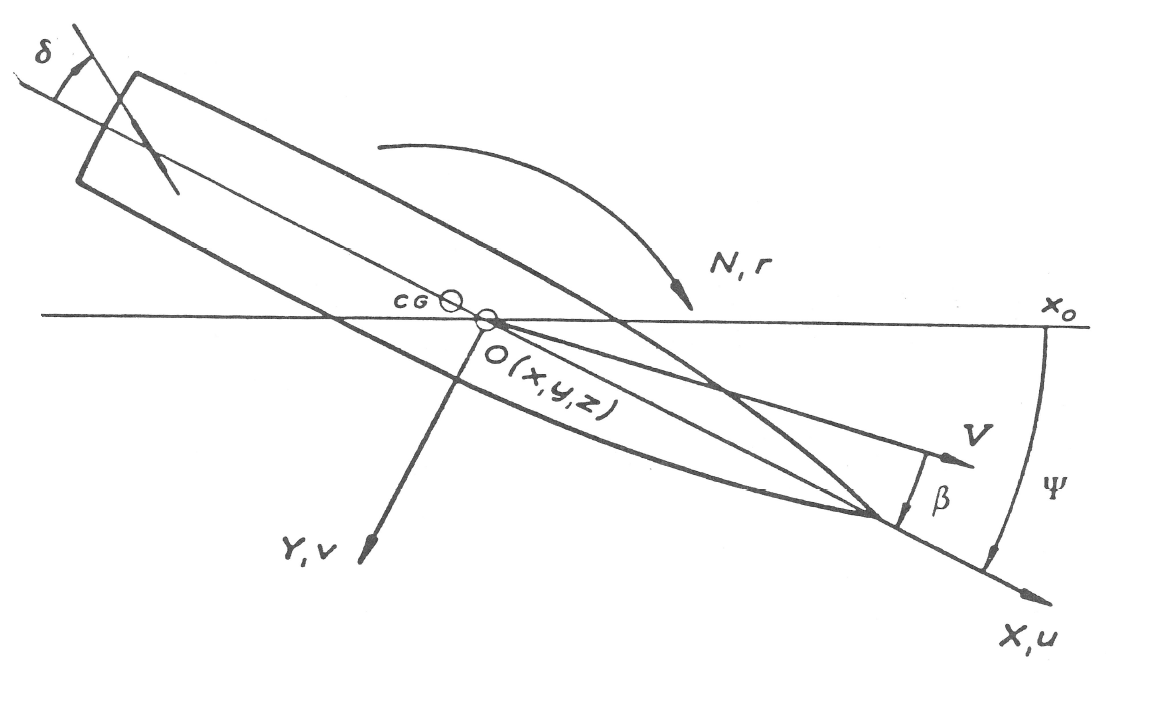
\includegraphics[width=0.8\textwidth]{kappa/images/coordinate_system.PNG}
    \caption{Reference frames.}
    \label{\detokenize{02.01_manoeuvring models:coordinate-system}}
\end{figure}

The manoeuvring equation can be described as \cite{fossen_handbook_2021},
\begin{equation}\label{equation:02.01_manoeuvring models:eqqsystem}
\begin{split}\displaystyle \left[\begin{matrix}- X_{\dot{u}} + m & 0 & 0\\0 & - Y_{\dot{v}} + m & - Y_{\dot{r}} + m x_{G}\\0 & - N_{\dot{v}} + m x_{G} & I_{z} - N_{\dot{r}}\end{matrix}\right] \left[\begin{matrix}\dot{u}\\\dot{v}\\\dot{r}\end{matrix}\right] = \left[\begin{matrix}m r^{2} x_{G} + m r v + \operatorname{X_{D}}{\left(u,v,r,\delta,thrust \right)}\\- m r u + \operatorname{Y_{D}}{\left(u,v,r,\delta,thrust \right)}\\- m r u x_{G} + \operatorname{N_{D}}{\left(u,v,r,\delta,thrust \right)}\end{matrix}\right]\end{split}
\end{equation}

\noindent where the first matrix describes the inertia of the ship in the surge, sway and yaw directions. The inertia in air is represented by the mass $m$ and moment of inertia $I_z$. The added mass in water is represented by: $X_{\dot{u}}$, $Y_{\dot{v}}$, $Y_{\dot{r}}$, $N_{\dot{v}}$ and $N_{\dot{r}}$. The hydrodynamic forces from the ship hull and rudder are desribed in the functions $X_D()$, $Y_D()$ and $N_D()$. The accelerations ($\dot{u}$, $\dot{v}$ and $\dot{r}$) can be solved from this equation,
\begin{equation}\label{equation:02.01_manoeuvring models:eqacc}
\begin{split}\displaystyle \dot{\nu} = \left[\begin{matrix}\dot{u}\\\dot{v}\\\dot{r}\end{matrix}\right] = \left[\begin{matrix}\frac{1}{- X_{\dot{u}} + m} & 0 & 0\\0 & - \frac{- I_{z} + N_{\dot{r}}}{S} & - \frac{- Y_{\dot{r}} + m x_{G}}{S}\\0 & - \frac{- N_{\dot{v}} + m x_{G}}{S} & - \frac{Y_{\dot{v}} - m}{S}\end{matrix}\right] \left[\begin{matrix}m r^{2} x_{G} + m r v + \operatorname{X_{D}}{\left(u,v,r,\delta,thrust \right)}\\- m r u + \operatorname{Y_{D}}{\left(u,v,r,\delta,thrust \right)}\\- m r u x_{G} + \operatorname{N_{D}}{\left(u,v,r,\delta,thrust \right)}\end{matrix}\right]\end{split}
\end{equation}
\sphinxAtStartPar
where \(S\) is a helper variable:
\begin{equation}\label{equation:02.01_manoeuvring models:eq_S}
\begin{split}\displaystyle S = - I_{z} Y_{\dot{v}} + I_{z} m + N_{\dot{r}} Y_{\dot{v}} - N_{\dot{r}} m - N_{\dot{v}} Y_{\dot{r}} + N_{\dot{v}} m x_{G} + Y_{\dot{r}} m x_{G} - m^{2} x_{G}^{2}\end{split}
\end{equation}
\sphinxAtStartPar

\noindent A state space model for manoeuvring can now be defined with six states:
\begin{equation}\label{equation:02.01_manoeuvring models:eq_x}
\begin{split}\displaystyle \mathbf{x} = \left[\begin{matrix}x_{0}\\y_{0}\\\Psi\\u\\v\\r\end{matrix}\right]\end{split}
\end{equation}
\noindent where $x_0$, $y_0$ and $\Psi$ are the global coordinates and heading of the ship and $u$, $v$ and $r$ are the velocities as seen in \autoref{\detokenize{02.01_manoeuvring models:coordinate-system}}.
The time derivative of this state \(\dot{\mathbf{x}}\) can be defined by a state transition \(f(\mathbf{x},\mathbf{c})\) using geometrical relations
how global coordinates \(x_0\), \(y_0\) and \(\Psi\) depend on \(u\), \(v\), and \(r\) viz.,
\begin{equation}\label{equation:02.01_manoeuvring models:eqf}
\begin{split}\displaystyle \dot{\mathbf{x}} = f(\mathbf{x},\mathbf{c}) + \mathbf{w}
                                          = \left[\begin{matrix}\dot{x_0}\\ \dot{y_0} \\ \dot{\Psi} \\\dot{u}\\\dot{v}\\\dot{r}\end{matrix}\right] + \mathbf{w}
                                          = \left[\begin{matrix}u \cos{\left(\Psi \right)} - v \sin{\left(\Psi \right)}\\u \sin{\left(\Psi \right)} + v \cos{\left(\Psi \right)}\\r\\\dot{u}\\\dot{v}\\\dot{r}\end{matrix}\right] + \mathbf{w}\end{split}
\end{equation}
\sphinxAtStartPar
where \(\mathbf{c}\) is control inputs (rudder angle \(\delta\) and thrust); the last three derivatives: \(\dot{u}\), \(\dot{v}\), \(\dot{r}\) are calculated with \autoref{equation:02.01_manoeuvring models:eqacc}.
\(\mathbf{w}\) is the process noise, i.e., the difference between the predicted state by the manoeuvring model and the true
state of the system. \(\mathbf{w}\) is unknown when the manoeuvring model is used for manoeuvre predictions and therefore normally
assumed to be zero, but it is an important factor when the manoeuvring model is used in the EKF (see \autoref{sec:datacleaning}).
The manoeuvring simulation can now be conducted by numerical integration of \autoref{equation:02.01_manoeuvring models:eqf}. The main difference between the manoeuvring model:s lies in how the hydrodynamic functions \(X_D(u,v,r,\delta,thrust)\), \(Y_D(u,v,r,\delta,thrust)\), \(N_D(u,v,r,\delta,thrust)\) are defined. These expressions are denoted in prime system ($X_D'$, $Y_D'$, $N_D'$) below for the various manoeuvring models: LVMM, AVMM and MAVMM.

{\normalfont \textbf{Linear vessel manoeuvring model (LVMM) \cite{matusiak_dynamics_2017}}}
\begin{equation}\label{equation:02.01_manoeuvring models:eqxlinear}
\begin{split}\begin{split}
\operatorname{X_{D}'}{\left(u',v',r',\delta\right)} = & X_{\delta} \delta + X_{r} r' + X_{u} u' + X_{v} v' 
\end{split}\end{split}
\end{equation}\begin{equation}\label{equation:02.01_manoeuvring models:eqylinear}
\begin{split}\begin{split}
\operatorname{Y_{D}'}{\left(u',v',r',\delta \right)} = & Y_{\delta} \delta + Y_{r} r' + Y_{u} u' + Y_{v} v' 
\end{split}\end{split}
\end{equation}\begin{equation}\label{equation:02.01_manoeuvring models:eqnlinear}
\begin{split}\begin{split}
\operatorname{N_{D}'}{\left(u',v',r',\delta \right)} = & N_{\delta} \delta + N_{r} r' + N_{u} u' + N_{v} v' 
\end{split}\end{split}
\end{equation}
\sphinxAtStartPar
{\normalfont \textbf{Abkowitz vessel manoeuvring model(AVMM) \cite{abkowitz_ship_1964}}}
\begin{equation}\label{equation:02.01_manoeuvring models:eqxabkowitz}
\begin{split}
\operatorname{X_{D}'}{\left(u',v',r',\delta,thrust' \right)} = & X_{\delta\delta} \delta^{2} + X_{r\delta} \delta r' + X_{rr} r'^{2} + X_{T} thrust' + X_{u\delta\delta} \delta^{2} u' \\ 
& + X_{ur\delta} \delta r' u' + X_{urr} r'^{2} u' + X_{uuu} u'^{3} + X_{uu} u'^{2} \\ 
& + X_{uv\delta} \delta u' v' + X_{uvr} r' u' v' + X_{uvv} u' v'^{2} \\
& + X_{u} u' + X_{v\delta} \delta v' + X_{vr} r' v' + X_{vv} v'^{2} 
\end{split}
\end{equation}

\begin{equation}\label{equation:02.01_manoeuvring models:eqyabkowitz}
\begin{split}\begin{split}
\operatorname{Y_{D}'}{\left(u',v',r',\delta,thrust' \right)} = & Y_{0uu} u'^{2} + Y_{0u} u' + Y_{0} + Y_{\delta\delta\delta} \delta^{3} + Y_{\delta} \delta + Y_{r\delta\delta} \delta^{2} r' + Y_{rr\delta} \delta r'^{2} \\ & + Y_{rrr} r'^{3} + Y_{r} r' + Y_{T\delta} \delta thrust' + Y_{T} thrust' + Y_{u\delta} \delta u' \\ & + Y_{ur} r' u' + Y_{uu\delta} \delta u'^{2} + Y_{uur} r' u'^{2} + Y_{uuv} u'^{2} v' + Y_{uv} u' v' \\ & + Y_{v\delta\delta} \delta^{2} v' + Y_{vr\delta} \delta r' v' + Y_{vrr} r'^{2} v' + Y_{vv\delta} \delta v'^{2} + Y_{vvr} r' v'^{2} \\ & + Y_{vvv} v'^{3} + Y_{v} v' 
\end{split}\end{split}
\end{equation}\begin{equation}\label{equation:02.01_manoeuvring models:eqnabkowitz}
\begin{split}\begin{split}
\operatorname{N_{D}'}{\left(u',v',r',\delta,thrust' \right)} = & N_{0uu} u'^{2} + N_{0u} u' + N_{0} + N_{\delta\delta\delta} \delta^{3} + N_{\delta} \delta + N_{r\delta\delta} \delta^{2} r' + N_{rr\delta} \delta r'^{2} \\ & + N_{rrr} r'^{3} + N_{r} r' + N_{T\delta} \delta thrust' + N_{T} thrust' + N_{u\delta} \delta u' \\ & + N_{ur} r' u' + N_{uu\delta} \delta u'^{2} + N_{uur} r' u'^{2} + N_{uuv} u'^{2} v' + N_{uv} u' v' \\ & + N_{v\delta\delta} \delta^{2} v' + N_{vr\delta} \delta r' v' + N_{vrr} r'^{2} v' + N_{vv\delta} \delta v'^{2} + N_{vvr} r' v'^{2} \\ & + N_{vvv} v'^{3} + N_{v} v' 
\end{split}\end{split}
\end{equation}
\sphinxAtStartPar
{\normalfont \textbf{Modified Abkowitz vessel manoeuvring model (MAVMM)}}
\newline
Only the most relevant coefficients in AVMM are included, as proposed in Paper \ref{pap:pit}.
\begin{equation}\label{equation:02.01_manoeuvring models:eqxmartinssimple}
\begin{split}\begin{split}
\operatorname{X_{D}'}{\left(u',v',r',\delta,thrust' \right)} = & X_{\delta\delta} \delta^{2} + X_{rr} r'^{2} + X_{T} thrust' + X_{uu} u'^{2} + X_{u} u' + X_{vr} r' v' 
\end{split}\end{split}
\end{equation}\begin{equation}\label{equation:02.01_manoeuvring models:eqymartinssimple}
\begin{split}\begin{split}
\operatorname{Y_{D}'}{\left(u',v',r',\delta,thrust' \right)} = & Y_{\delta} \delta + Y_{r} r' + Y_{T\delta} \delta thrust' + Y_{T} thrust' + Y_{ur} r' u' \\ & + Y_{u} u' + Y_{vv\delta} \delta v'^{2} + Y_{v} v' 
\end{split}\end{split}
\end{equation}\begin{equation}\label{equation:02.01_manoeuvring models:eqnmartinssimple}
\begin{split}\begin{split}
\operatorname{N_{D}'}{\left(u',v',r',\delta,thrust' \right)} = & N_{\delta} \delta + N_{r} r' + N_{T\delta} \delta thrust' + N_{T} thrust' + N_{ur} r' u' + N_{u} u' \\ & + N_{vv\delta} \delta v'^{2} + N_{v} v' 
\end{split}\end{split}
\end{equation}
\sphinxAtStartPar
The hydrodynamic functions above are expressed using nondimensional units with the prime system, denoted by the prime symbol (\('\)). The quantities are expressed in the prime system, using the denominators in Tab.\ref{tab:my_label}. For instance, surge linear velocity \(u\) can be expressed in the prime system as seen in \autoref{equation:02.01_manoeuvring models:eqprime} using the linear velocity denominator.
\begin{equation}\label{equation:02.01_manoeuvring models:eqprime}
\begin{split}\displaystyle u'=\frac{u}{V}\end{split}
\end{equation}
\sphinxAtStartPar
Equations can either be written in the prime or regular Standard Institute (SI) system. The hydrodynamic derivatives are always expressing forces in the prime system as function of state variables. The (\('\)) sign is therefore implicit and not written out as seen in \autoref{equation:02.01_manoeuvring models:eqderivativeprime}.
\begin{equation}\label{equation:02.01_manoeuvring models:eqderivativeprime}
\begin{split}\displaystyle Y_{\delta'}'=\frac{\partial Y_D'}{\partial \delta'} := Y_{\delta} \end{split}
\end{equation}
\sphinxAtStartPar
The exceptions are the added masses (\(X_{\dot{u}}\), \(Y_{\dot{v}}\), \(Y_{\dot{r}}\), \(N_{\dot{v}}\) and \(N_{\dot{r}}\)) which are expressed in both Prime system or the regular SI system where the (\('\)) sign is therefore
explicitly stated.
There is however a great benefit in expressing the hydrodynamic forces in the prime system. The forces are often nonlinear due to a quadratic relation to the flow velocity, as seen in \autoref{equation:02.01_manoeuvring models:eqquadraticsi}.
\begin{equation}\label{equation:02.01_manoeuvring models:eqquadraticsi}
\begin{split}\displaystyle Y_{D}=Y_{\delta} \cdot \delta \cdot \frac{L^2V^2\rho}{2}\end{split}
\end{equation}
which becomes linear when expressed in the prime system as seen in \autoref{equation:02.01_manoeuvring models:eqquadraticprime}.
\begin{equation}\label{equation:02.01_manoeuvring models:eqquadraticprime}
\begin{split}\displaystyle Y_{D}'=Y_{\delta} \cdot \delta'\end{split}
\end{equation}


\begin{table}[]
\caption{Prime system denominators.}
\label{tab:prime-system-denominators}
\centering
\label{tab:my_label}
\begin{tabular}{c c}
\toprule
Quantity &
Denominators
\\
\hline

angle
&

\(1\)
\\


angular
acceleration
&

\(\frac{V^{2}}{L^{2}}\)
\\


angular
velocity
&

\(\frac{V}{L}\)
\\


area
&

\(L^{2}\)
\\


density
&

\(\frac{\rho}{2}\)
\\


force
&

\(\frac{L^{2} V^{2} \rho}{2}\)
\\


frequency
&

\(\frac{V}{L}\)
\\


inertia
moment
&

\(\frac{L^{5} \rho}{2}\)
\\


length
&

\(L\)
\\


linear
acceleration
&

\(\frac{V^{2}}{L}\)
\\


linear
velocity
&

\(V\)
\\


mass
&

\(\frac{L^{3} \rho}{2}\)
\\


moment
&

\(\frac{L^{3} V^{2} \rho}{2}\)
\\


time
&

\(\frac{L}{V}\)
\\


volume
&

\(L^{3}\)
\\
\bottomrule

\end{tabular}


\end{table}

\subsection{The propeller model}
\label{\detokenize{02.10_propeller_model:the-propeller-model}}\label{\detokenize{02.10_propeller_model::doc}}

A propeller model is developed based on Manoeuvring Modeling Group (MMG) model \cite{yasukawa_introduction_2015-1} where the thrust is expressed as:
\begin{equation}\label{equation:02.10_propeller_model:eqT}
\begin{split}\displaystyle thrust = D^{4} K_{T} n^{2} \rho\end{split}
\end{equation}

and the thrust coefficient \(K_T\) is modelled as a second order polynomial:
\begin{equation}\label{equation:02.10_propeller_model:eqkt}
\begin{split}\displaystyle K_{T} = J^{2} k_{2} + J k_{1} + k_{0}\end{split}
\end{equation}

The advance ratio \(J\) is calculated as:
\begin{equation}\label{equation:02.10_propeller_model:eqJ}
\begin{split}\displaystyle J = \frac{u \left(1 - w_{p}\right)}{D n}\end{split}
\end{equation}

where \(D\) is propeller diameter, \(n\) is propeller speed and \(w_p\) is the wake fraction at an oblique inflow to the propeller from the drift angle and the yaw rate. A semi\sphinxhyphen{}empirical formula for \(w_p\) is provided in the MMG model. As an alternative, a simple polynomial is proposed in \autoref{equation:02.10_propeller_model:eqpropellermodel}.
\begin{equation}\label{equation:02.10_propeller_model:eqpropellermodel}
\begin{split}\displaystyle w_{p} = C_{1} \delta + C_{2} \delta^{2} + C_{3} \beta_{p}^{2} + C_{4} u + w_{p0}\end{split}
\end{equation}

\(w_p\) is modeled as a function of rudder angle \(\delta\), to include wake influence from the rudder and ship speed \(u\), to include a speed dependency. The influence from drift angle \(\beta\) and yaw rate \(r\) is expressed by \(\beta_p\) in \autoref{equation:02.10_propeller_model:eqbetap}.
\begin{equation}\label{equation:02.10_propeller_model:eqbetap}
\begin{split}\beta_p=\beta - \frac{r}{V} \cdot x_p \end{split}
\end{equation}

Where \(x_p\) is the propeller longitudinal position and \(w_{p0}\) is the regular Taylor wake fraction, applicable to straight ahead steaming with no rudder angle. Similar to the MMG propeller model, two sets of parameters \(C_1\)-\(C_4\) should be used in the propeller model depending on the sign of \(\beta_p\).